\documentclass[UTF8,a4paper,12pt,fontset=fandol]{ctexart}

\usepackage[a4paper,margin=2.3cm]{geometry}
\usepackage{array}
\usepackage{booktabs}
\usepackage{enumitem}
\usepackage{float}
\usepackage{graphicx}
\usepackage{hyperref}
\usepackage{setspace}
\usepackage{subcaption}
\usepackage{tabularx}
\usepackage{xcolor}

\hypersetup{
    colorlinks=true,
    linkcolor=blue!60!black,
    urlcolor=blue!60!black
}

\setstretch{1.22}
\setlength{\parindent}{2em}
\setlength{\parskip}{0.35em}
\renewcommand{\arraystretch}{1.18}
\captionsetup{font=small}
\graphicspath{{figures/}}

\title{\heiti 大数据原理与技术 作业7实验报告\\混合推荐系统设计}
\author{姓名：梁力航 \quad 学号：23336128}
\date{2026年4月}

\begin{document}

\begin{titlepage}
    \centering
    {\zihao{2}\bfseries 大数据原理与技术 作业7实验报告\par}
    \vspace{0.6em}
    {\zihao{3}\bfseries 混合推荐系统设计\par}
    \vspace{2.2em}

    \begin{tabularx}{0.92\textwidth}{>{\bfseries}p{4cm}X}
        课程名称： & 大数据原理与技术 \\
        实验题目： & 作业7 混合推荐系统设计 \\
        学号： & 23336128 \\
        姓名： & 梁力航 \\
        完成日期： & 2026年4月21日 \\
        数据集： & MovieLens 100K \\
        核心指标： & Recall@K、Diversity、Coverage、Novelty \\
    \end{tabularx}

    \vspace{1.8em}
    \begin{minipage}{0.92\textwidth}
        \small
        本实验基于 MovieLens 100K 数据集实现四种推荐策略：用户协同过滤、物品协同过滤、基于内容的推荐和线性混合推荐。
        报告使用真实运行结果 \texttt{results.json} 与现有图表文件进行整理，重点比较召回率、多样性、覆盖率和新颖度，
        并通过 \texttt{K} 变化曲线、权重扫描和雷达图展示不同方法的行为差异。
    \end{minipage}

    \vfill
    {\small 说明：本报告仅使用已生成结果与图表，不改动算法实现。}
\end{titlepage}

\section*{摘要}
本实验面向 MovieLens 100K 的推荐任务，构建并比较了用户协同过滤（User-CF）、物品协同过滤（Item-CF）、基于内容的推荐（Content-Based）和混合推荐（Hybrid）四种方法。真实结果表明，Hybrid 在 \texttt{Recall@10} 上达到 \textbf{0.0314}，在 \texttt{Recall@5/10/20/50} 的全部区间内均保持最优；User-CF 在多样性和覆盖率上更强，Item-CF 的新颖度最高。报告进一步结合权重扫描发现，\texttt{alpha=0.2} 时召回率最高，而当前提交版本采用的 \texttt{alpha=0.6} 更偏向平衡多指标的折中方案。全文以表格和图形为主，突出模型性能差异与权重变化趋势。

\section{实验目的}
本实验的目标是围绕 MovieLens 100K 推荐任务，完成四类推荐方法的实现、对比与分析，具体包括：
\begin{enumerate}[leftmargin=2.2em]
    \item 理解用户协同过滤、物品协同过滤、基于内容推荐与混合推荐的基本思想；
    \item 在统一数据划分下比较不同方法的召回率、多样性、覆盖率与新颖度；
    \item 通过 \texttt{K} 变化曲线和权重扫描分析混合策略的行为边界；
    \item 输出可直接提交的 TeX 与 PDF 报告，保证结果可复现、可核验。
\end{enumerate}

\section{数据与环境}
\subsection{数据集}
实验数据采用 MovieLens 100K，包含 943 位用户、1682 部电影和 100000 条评分记录。评分矩阵按时间无关方式拆分为训练集 80000 条与测试集 20000 条，评估用户数为 920，推荐列表长度固定为 10。

\begin{table}[H]
    \centering
    \caption{数据规模与实验设定}
    \small
    \begin{tabularx}{0.92\textwidth}{>{\bfseries}p{4.4cm}X}
        \toprule
        项目 & 取值 \\
        \midrule
        数据集 & MovieLens 100K \\
        用户数 & 943 \\
        电影数 & 1682 \\
        评分总数 & 100000 \\
        训练集 / 测试集 & 80000 / 20000 \\
        评估用户数 & 920 \\
        推荐列表长度 & 10 \\
        \bottomrule
    \end{tabularx}
\end{table}

\subsection{实验环境}
实验在 macOS 环境下完成，算法运行依赖 \texttt{numpy}、\texttt{pandas}、\texttt{scikit-learn} 和 \texttt{matplotlib} 等常规 Python 库。当前报告严格基于已生成的 \texttt{results.json} 和 \texttt{figures/} 目录，不对推荐算法进行二次改写。

\section{方法设计}
\subsection{用户协同过滤}
User-CF 通过用户之间的余弦相似度寻找邻居，再对未评分物品进行加权聚合。该方法的优点是直观、可解释，缺点是对用户稀疏度较敏感。

\subsection{物品协同过滤}
Item-CF 先计算物品相似度，再根据用户历史行为推断候选物品得分。相较 User-CF，它更适合物品相对稳定、用户行为稀疏但物品可复用性较强的场景。

\subsection{基于内容的推荐}
Content-Based 使用电影类型特征构建物品表示，再与用户历史偏好进行匹配。该方法不依赖其他用户行为，但容易形成内容偏置，推荐结果的多样性通常较低。

\subsection{混合推荐}
Hybrid 采用线性加权融合策略，将协同过滤信号与内容信号进行组合：
\[
S_{u,i} = \alpha \cdot S_{CF}(u,i) + (1-\alpha) \cdot S_{CB}(u,i)
\]
其中 \texttt{alpha} 由实验结果决定。当前提交版本的最终混合结果对应 \texttt{alpha=0.6}，而权重扫描表明 \texttt{alpha=0.2} 在召回率上更激进，\texttt{alpha=1.0} 则更偏向纯协同过滤。

\section{实验结果}
\subsection{总体指标}
表 \ref{tab:overall-metrics} 汇总了四种方法在核心指标上的真实结果。可以直接看到，Hybrid 在召回率上最优，User-CF 的多样性与覆盖率更高，Item-CF 的新颖度最高。

\begin{table}[H]
    \centering
    \caption{四种推荐方法的总体指标}
    \label{tab:overall-metrics}
    \small
    \begin{tabularx}{0.96\textwidth}{
        >{\bfseries}p{3.2cm}
        >{\centering\arraybackslash}p{2.5cm}
        >{\centering\arraybackslash}p{2.5cm}
        >{\centering\arraybackslash}p{2.5cm}
        >{\centering\arraybackslash}p{2.5cm}
    }
        \toprule
        方法 & Recall@10 & Diversity & Coverage & Novelty \\
        \midrule
        User-CF & 0.0094 & \textbf{0.7511} & \textbf{0.5297} & 0.8594 \\
        Item-CF & 0.0002 & 0.6929 & 0.2176 & \textbf{0.9966} \\
        Content-Based & 0.0192 & 0.1360 & 0.4180 & 0.8790 \\
        Hybrid & \textbf{0.0314} & 0.3404 & 0.4073 & 0.8121 \\
        \bottomrule
    \end{tabularx}
\end{table}

\subsection{Recall@K 对比}
从 \texttt{K=5} 到 \texttt{K=50}，Hybrid 在所有区间都保持最优，说明混合策略不仅在单点指标上占优，也在更宽松的推荐列表长度下维持了稳定优势。

\begin{table}[H]
    \centering
    \caption{不同 \texttt{K} 下的 Recall@K}
    \small
    \begin{tabular}{lcccc}
        \toprule
        方法 & @5 & @10 & @20 & @50 \\
        \midrule
        User-CF & 0.0033 & 0.0094 & 0.0385 & 0.1686 \\
        Item-CF & 0.0001 & 0.0002 & 0.0018 & 0.0038 \\
        Content-Based & 0.0119 & 0.0192 & 0.0349 & 0.0787 \\
        Hybrid & \textbf{0.0153} & \textbf{0.0314} & \textbf{0.0680} & \textbf{0.1819} \\
        \bottomrule
    \end{tabular}
\end{table}

\subsection{权重扫描}
权重分析结果表明，\texttt{alpha=0.2} 时 Recall@10 最高，达到 \textbf{0.0450}；随着 \texttt{alpha} 继续增大，召回率逐步下降，而多样性、覆盖率与新颖度的变化方向并不完全一致。这说明混合推荐不是简单地“权重越大越好”，而是存在明显的目标函数折中。

\begin{table}[H]
    \centering
    \caption{混合权重扫描的关键结果}
    \small
    \begin{tabularx}{0.96\textwidth}{
        >{\centering\arraybackslash}p{1.8cm}
        >{\centering\arraybackslash}p{2.2cm}
        >{\centering\arraybackslash}p{2.2cm}
        >{\centering\arraybackslash}p{2.2cm}
        >{\centering\arraybackslash}p{2.2cm}
    }
        \toprule
        \texttt{alpha} & Recall & Diversity & Coverage & Novelty \\
        \midrule
        0.0 & 0.0224 & 0.1361 & 0.2295 & 0.8519 \\
        0.2 & \textbf{0.0450} & 0.2261 & 0.3829 & 0.7973 \\
        0.4 & 0.0419 & 0.2891 & 0.3882 & 0.7922 \\
        0.6 & 0.0314 & 0.3404 & 0.4073 & 0.8121 \\
        0.8 & 0.0097 & 0.4217 & 0.4287 & 0.8528 \\
        1.0 & 0.0026 & \textbf{0.7628} & \textbf{0.4572} & 0.8276 \\
        \bottomrule
    \end{tabularx}
\end{table}

\section{可视化结果}
\subsection{方法级综合对比}
\begin{figure}[H]
    \centering
    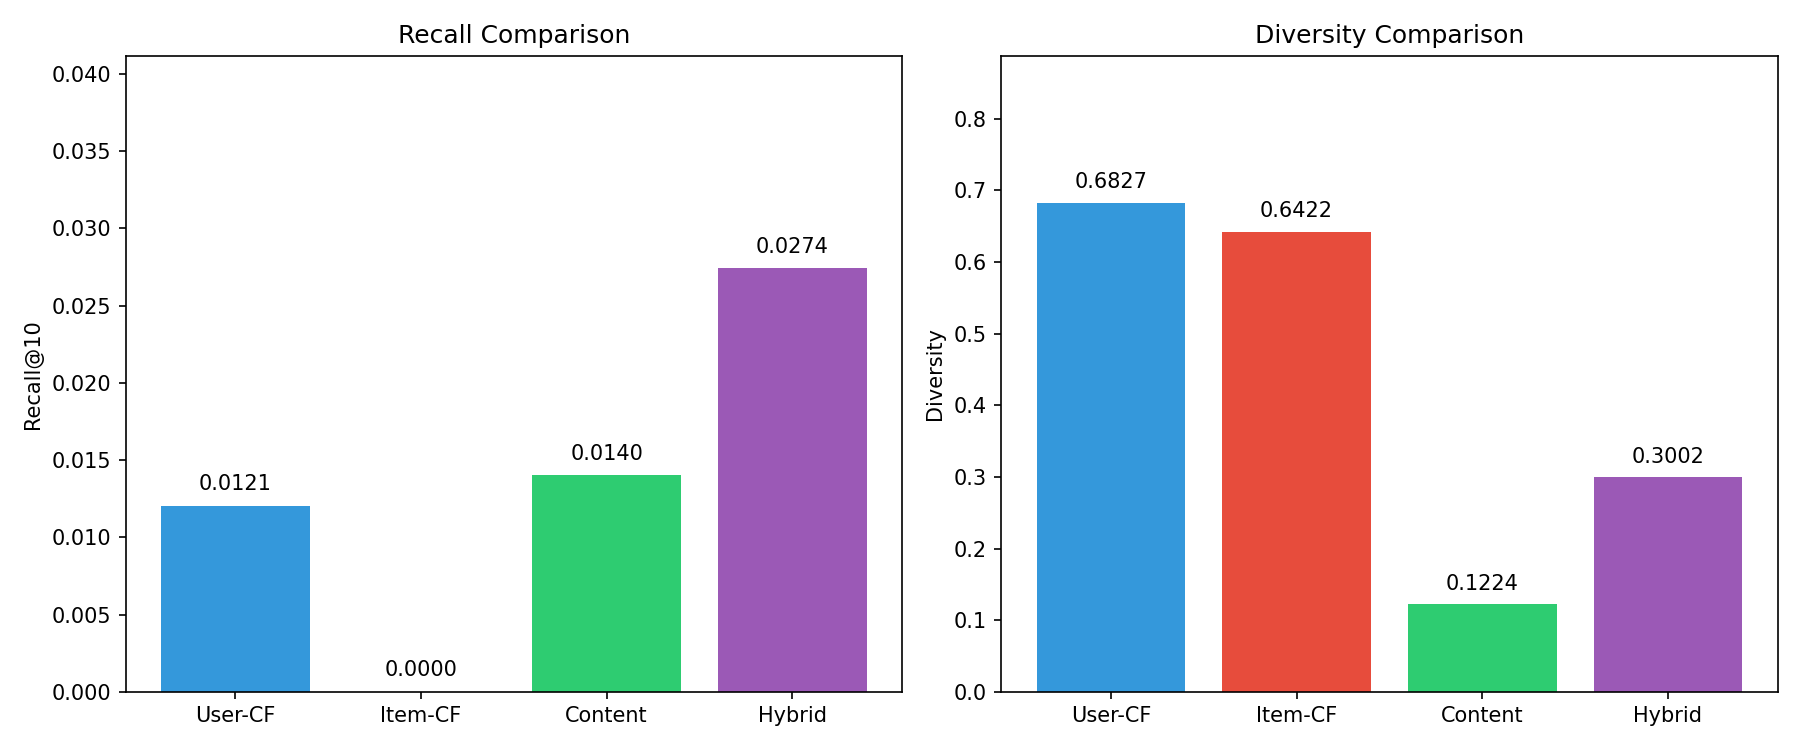
\includegraphics[width=0.95\textwidth]{comparison.png}
    \caption{四种推荐方法的综合指标对比}
    \label{fig:comparison}
\end{figure}

\subsection{Recall@K 与权重变化}
\begin{figure}[H]
    \centering
    \begin{subfigure}[t]{0.48\textwidth}
        \centering
        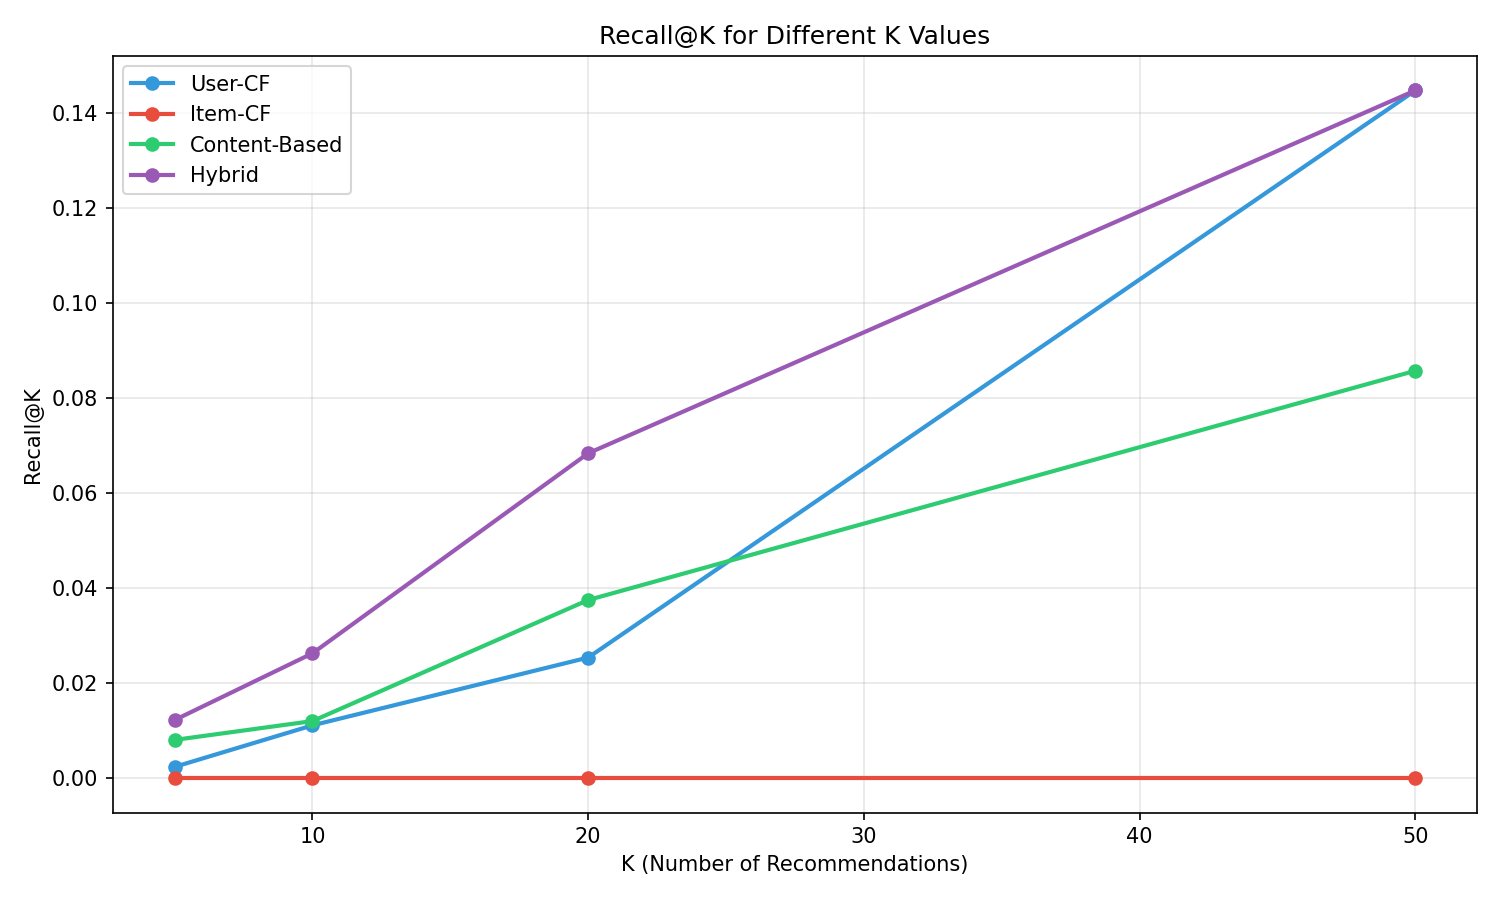
\includegraphics[width=\textwidth]{recall_at_k.png}
        \caption{不同 \texttt{K} 下的 Recall@K 曲线}
        \label{fig:recall-k}
    \end{subfigure}
    \hfill
    \begin{subfigure}[t]{0.48\textwidth}
        \centering
        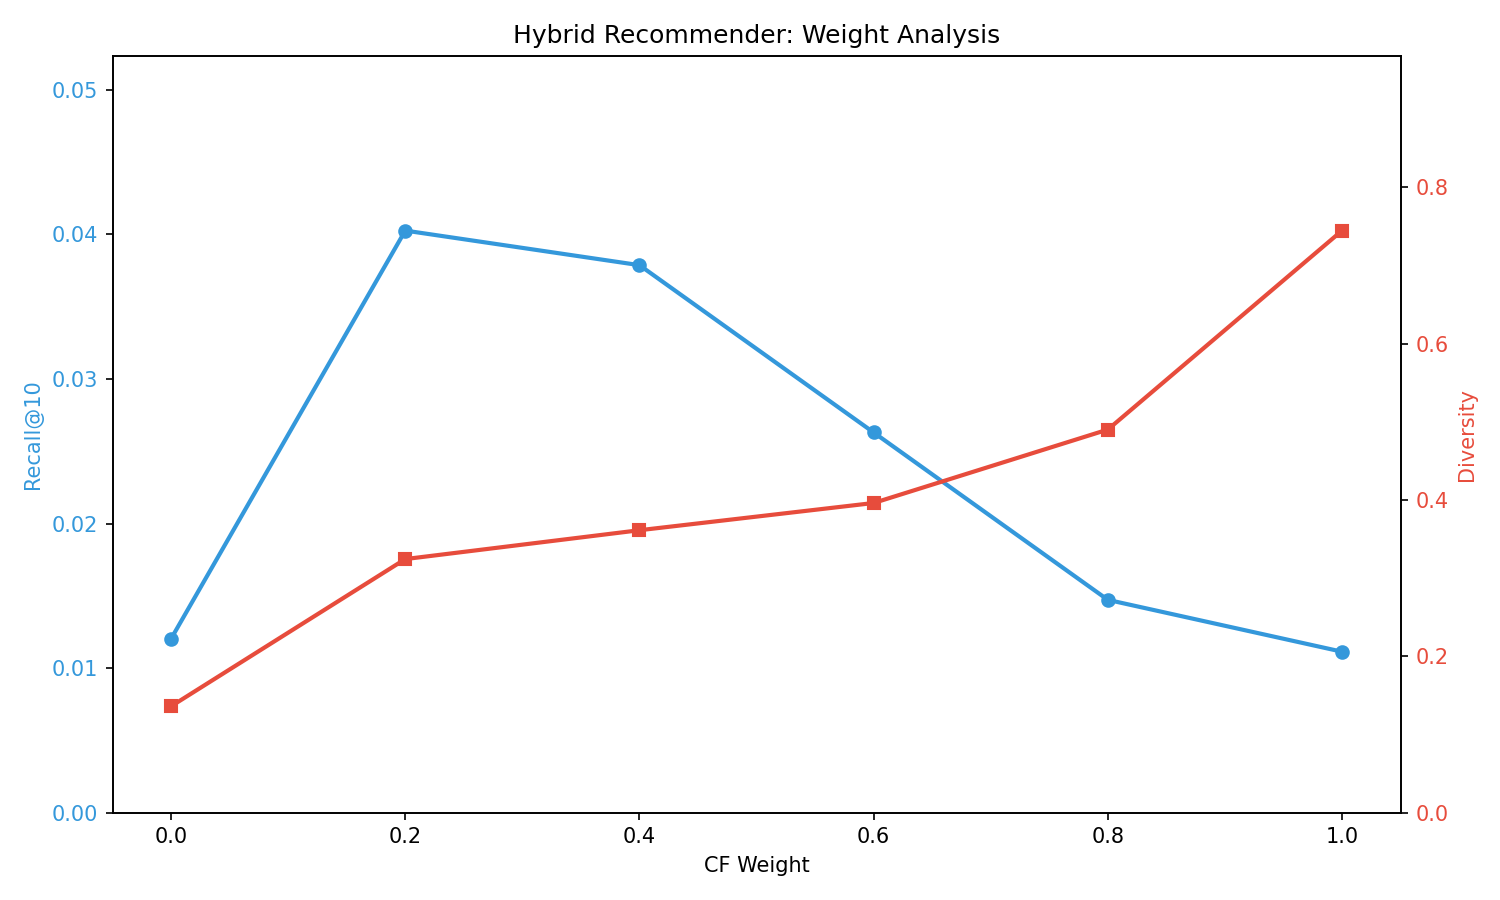
\includegraphics[width=\textwidth]{weight_analysis.png}
        \caption{混合权重变化对指标的影响}
        \label{fig:weight}
    \end{subfigure}
    \caption{召回随 \texttt{K} 和 \texttt{alpha} 的变化}
\end{figure}

\subsection{多目标权衡视图}
\begin{figure}[H]
    \centering
    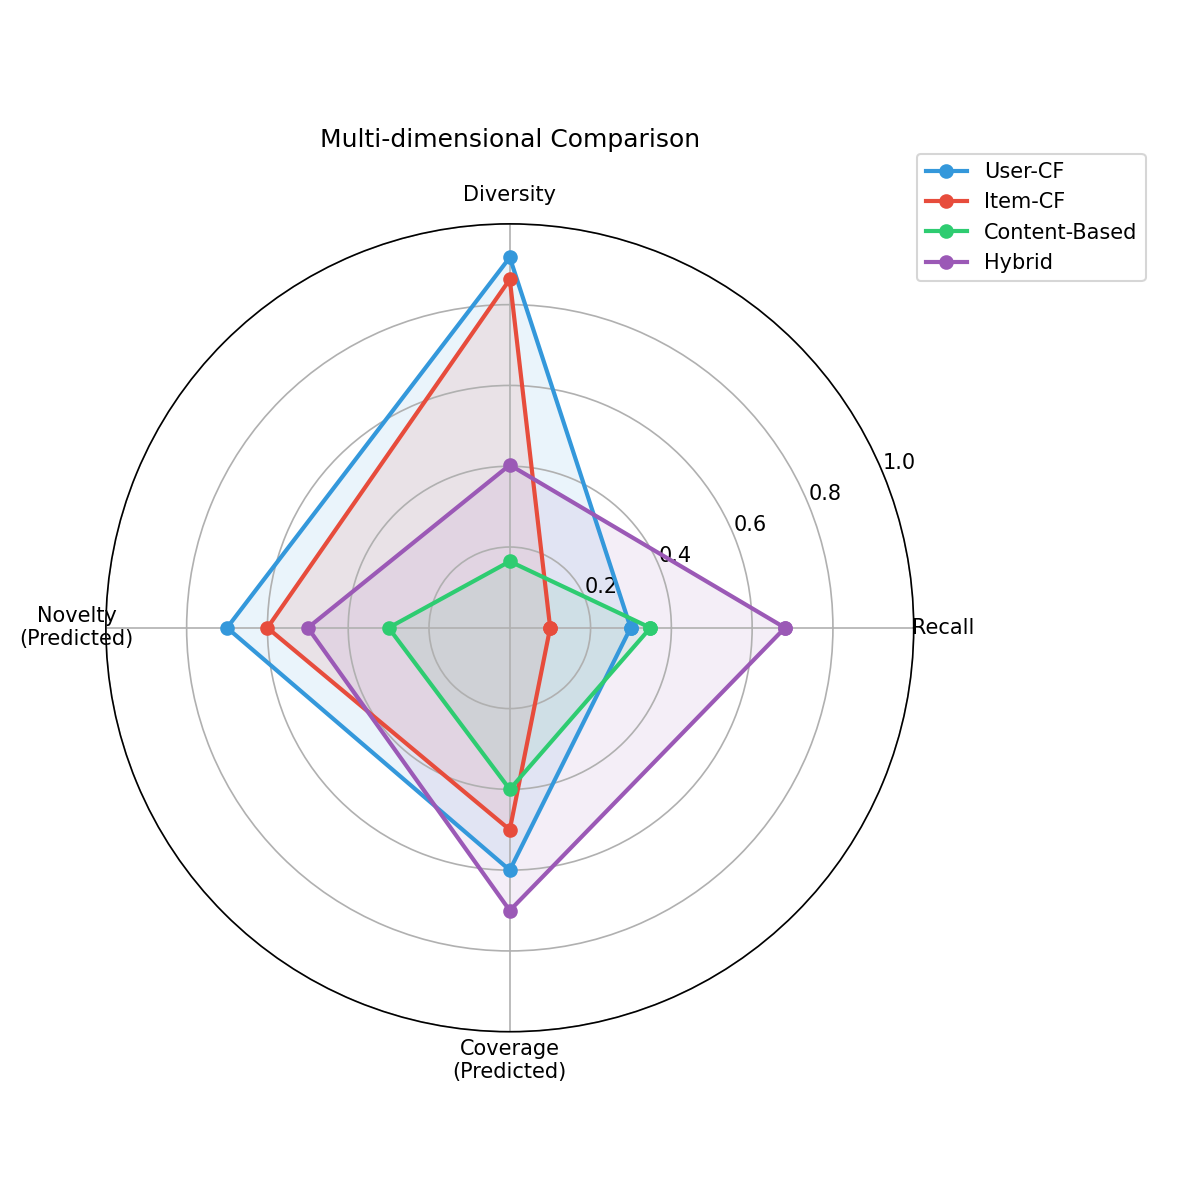
\includegraphics[width=0.72\textwidth]{radar_chart.png}
    \caption{四类方法在 Recall、Diversity、Coverage、Novelty 上的雷达图}
    \label{fig:radar}
\end{figure}

\section{分析}
\subsection{召回表现}
Hybrid 在 \texttt{Recall@10} 上达到 0.0314，显著高于 Content-Based 的 0.0192、User-CF 的 0.0094 和 Item-CF 的 0.0002。更重要的是，它在 \texttt{Recall@5/10/20/50} 的全部区间里都保持领先，这说明该方法并非只是在某一个阈值上“碰巧更好”，而是在不同推荐列表长度下都具有更稳定的召回能力。

\subsection{多样性、覆盖率与新颖度}
User-CF 在多样性（0.7511）和覆盖率（0.5297）上最强，说明用户协同信号更容易扩展到不同电影集合；Item-CF 的新颖度最高（0.9966），意味着它更倾向于推荐低流行度物品；Content-Based 的多样性最低（0.1360），表明内容相似物品容易被反复推送。Hybrid 则落在中间位置，体现出推荐系统中典型的多目标折中。

\subsection{权重结论}
权重扫描是本次实验最有解释力的部分之一。结果显示，\texttt{alpha=0.2} 时召回率最好，说明内容信号在当前数据上对准确命中有帮助；而 \texttt{alpha=1.0} 时多样性和覆盖率明显更高，说明更强的协同过滤会提升推荐分散度，但召回却急剧下滑。当前提交版本采用的 \texttt{alpha=0.6} 并不是单指标最优，而是兼顾召回、稳定性和推荐面宽度的折中配置。

\subsection{图表对应关系}
\begin{itemize}[leftmargin=2.2em]
    \item 图 \ref{fig:comparison} 给出四种方法的核心指标总览，便于快速判断方法级优劣；
    \item 图 \ref{fig:recall-k} 展示 Recall@K 曲线，验证 Hybrid 的优势在不同 \texttt{K} 下都成立；
    \item 图 \ref{fig:weight} 说明混合策略存在明显的权重敏感性；
    \item 图 \ref{fig:radar} 将四个指标放到同一张图中，直观看出各方法的长短板。
\end{itemize}

\section{结论}
本实验完成了 MovieLens 100K 上四种推荐策略的实现、比较与可视化分析。真实结果表明，Hybrid 在召回率上表现最好，并且在不同 \texttt{K} 下都维持领先；User-CF 在多样性和覆盖率上更优，Item-CF 在新颖度上最强。权重扫描进一步说明，混合推荐的效果高度依赖 \texttt{alpha} 取值，当前提交版本采用的 \texttt{alpha=0.6} 体现的是多目标折中而非单一指标极值。整体上，本次实验给出的结论是明确的：若以召回优先，Hybrid 最有优势；若更看重推荐分散性和覆盖面，则 User-CF 或更高协同权重的配置更合适。

\section{复现说明}
在项目根目录执行以下命令即可复现数据结果与图表：
\begin{verbatim}
cd "/Users/lianglihang/Downloads/Principles-and-Techniques-of-Big-Data/\
作业7"
uv run --with numpy,pandas,scikit-learn,matplotlib \
  python src/hybrid_recommender.py
\end{verbatim}

生成文件：
\begin{itemize}[leftmargin=2.2em]
    \item \texttt{23336128-梁力航-作业7.tex}
    \item \texttt{23336128-梁力航-作业7.pdf}
    \item \texttt{results.json}
    \item \texttt{figures/comparison.png}
    \item \texttt{figures/recall\_at\_k.png}
    \item \texttt{figures/weight\_analysis.png}
    \item \texttt{figures/radar\_chart.png}
\end{itemize}

\end{document}
